\documentclass{beamer}
\usetheme{Madrid}

\usepackage[utf8]{inputenc}

\usepackage{tikz}
\usetikzlibrary{shapes.geometric,shapes.arrows,decorations.pathmorphing}
\usetikzlibrary{matrix,chains,scopes,positioning,arrows,fit}
\usepackage{varwidth}

\usepackage{multicol}

\usepackage{listings}
\usepackage{color}
\definecolor{lightgray}{rgb}{.9,.9,.9}
\definecolor{darkgray}{rgb}{.4,.4,.4}
\definecolor{purple}{rgb}{0.65, 0.12, 0.82}
\lstdefinelanguage{JavaScript}{
  keywords={break, case, catch, continue, debugger, default, delete, do, else, false, finally, for, function, if, in, instanceof, new, null, return, switch, this, throw, true, try, typeof, var, void, while, with},
  morecomment=[l]{//},
  morecomment=[s]{/*}{*/},
  morestring=[b]',
  morestring=[b]",
  ndkeywords={class, export, boolean, throw, implements, import, this},
  keywordstyle=\color{blue}\bfseries,
  ndkeywordstyle=\color{darkgray}\bfseries,
  identifierstyle=\color{black},
  commentstyle=\color{purple}\ttfamily,
  stringstyle=\color{red}\ttfamily,
  sensitive=true
}

\lstset{
   language=JavaScript,
   backgroundcolor=\color{white},
   extendedchars=true,
   basicstyle=\small,
   showstringspaces=false,
   showspaces=false,
   tabsize=2,
   breaklines=true,
   showtabs=false,
   captionpos=b
}
 
%Information to be included in the title page:
\title[JSAP Tutorial]{JSAP Tutorial: Build and deploy web audio effects}
 
\author[Jillings and Stables]% (optional, for multiple authors)
{Nicholas Jillings \and Ryan Stables}
 
\institute[BCU]
{
  Digital Media Technology Lab\\
  Birmingham City University\\
  Curzon Street, Birmingham, UK
}
 
\date[WAC 2017] % (optional)
{3rd Web Audio Conference (WAC-2017), August 21--23, 2017}

\begin{document}
 
\frame{\titlepage}

\begin{frame}
\frametitle{Introduction}

Aims of this tutorial:
\begin{itemize}
\item Learn how the JSAP standard works
\item How to deploy JSAP into your projects
\item Build your first JSAP plugin (start thinking of ideas).
\item Learn how to load plugins into the host and operate
\end{itemize}

\end{frame}

\begin{frame}
\frametitle{JSAP Overview}
Each JSAP plugin is made up of several objects:
\begin{itemize}
\item \texttt{BasePlugin} - The inherited object which defines every required interaction of the JSAP instance.
\begin{itemize}
\item \texttt{ParameterManager} - Built and accessed as \texttt{this.parameters}, holds all the constructors for parameters and interface for manipulating them.
\item \texttt{PluginFeatureInterface} - Allows for sharing of audio features between plugins (not going to cover today).
\item \texttt{PluginUserInterface} - For building of plugin GUI. Can hold several suitable options and interfaces.
\end{itemize}
\end{itemize}
These are all built for you on construction.
\end{frame}

\begin{frame}
\frametitle{Get JSAP}
Please clone the following GitHub resource:\\
\url{https://github.com/nickjillings/jsap-wac-tutorial}\\
This will give you the latest JSAP, jsap-plugins and jsap-sandbox environments.\\
Then open the file \texttt{helloworld.js} in your editor.\\
\end{frame}

\begin{frame}[fragile]
\frametitle{Get JSAP}
\begin{lstlisting}[language=javascript]
var HelloWorld = function (factory, owner) {

    // This attaches the base plugin items to the Object
    BasePlugin.call(this, factory, owner);

    /* USER MODIFIABLE BEGIN */

    /* USER MODIFIABLE END */
};

// Also update the prototype function here!
HelloWorld.prototype = Object.create(BasePlugin.prototype);
HelloWorld.prototype.constructor = HelloWorld;
HelloWorld.prototype.name = "HelloWorld";
HelloWorld.prototype.version = "1.0.0";
HelloWorld.prototype.uniqueID = "JSHW";
\end{lstlisting}


\end{frame}

\begin{frame}
\frametitle{Next Steps}
HelloWorld is just the shell, right now it is empty! We need to fill it with:
\begin{enumerate}
\item A graph! What Web Audio Nodes should we add? What effect shall we create?
\item Parameters! How shall an end user interact with the plugin? What are the parameter names? How do they map onto our nodes?
\item GUI! How shall our plugin look? (We'll cheat today and let the sandbox host manage that).
\item I/O. What is the audio insert point and exit point.
\end{enumerate}

\end{frame}

\begin{frame}[fragile]
\frametitle{Defining the graphs}
The audio context is given to all plugins as \texttt{this.context}.\\
Can easily build a simply \texttt{GainNode} by \texttt{var node = this.context.createGain();}\\
Inside the plugin, encapsulation allows us to build our nodes in private.
\begin{lstlisting}[language=javascript]
    /* USER MODIFIABLE BEGIN */
    var node = this.context.createGain();
    /* USER MODIFIABLE END */
\end{lstlisting}
\end{frame}

\begin{frame}
\frametitle{Adding Parameters}
JSAP supports several parameter types:
\begin{itemize}
\item \texttt{NumberParameter}
    \begin{itemize}
    \item Standard numerical range parameter control
    \item Can set min/max ranges
    \item \texttt{this.parameters.createNumberParameter}
    \end{itemize}
\item \texttt{StringParameter}
    \begin{itemize}
    \item Send / Receive a string with the plugin
    \item Can set maximum string length
    \item \texttt{this.parameters.createStringParameter}
    \end{itemize}
\item \texttt{ButtonParameter}
    \begin{itemize}
    \item Trigger Parameter
    \item Same behaviour as HTML\texttt{<button>} element
    \item \texttt{this.parameters.createButtonParameter}
    \end{itemize}
\item \texttt{SwitchParameter}
\begin{itemize}
    \item Iterable parameter
    \item Similar to dropdown. Fixed number of interactions
    \item Can pass through (up/down, next/prev etc) or set to specific value
    \item \texttt{this.parameters.createSwitchParameter}
    \end{itemize}
\end{itemize}
\end{frame}

\begin{frame}
\frametitle{Adding Parameters}
All parameters have a similar constructor:\\
\texttt{createNumberParameter(name, default, min, max);}\\
\texttt{createStringParameter(name, default, maxLength);}\\
\texttt{createButtonParameter(name, default);}\\
\texttt{createSwitchParameter(name, default, minState, maxState);}\\
Must define the name, a unique string to identify the parameter, and the default value (what to initialise it to).

\end{frame}


\begin{frame}[fragile]
\frametitle{Adding Parameters}
Let's add our parameter to our gain node:
\begin{lstlisting}[language=javascript]
    /* USER MODIFIABLE BEGIN */
    var node = this.context.createGain();
    var gain_parameter = this.parameters.createNumberParameter("gain", 0, -12, 12);
    /* USER MODIFIABLE END */
\end{lstlisting}
\end{frame}

\begin{frame}[fragile]
\frametitle{Adding Parameters}
Now we must bind the parameter. It must do something! Two ways to do this:
\begin{enumerate}
\item If a parameter maps to one node parameter, use \texttt{bindToAudioParam}
\begin{itemize}
\item For instance: \texttt{gain\_parameter.bindToAudioParam(node.gain)}.
\end{itemize}
\item If one parameter to many node parameters, or sharing a node parameter, use \texttt{trigger} to write function
\begin{itemize}
\item For instance:
\end{itemize}
\end{enumerate}
\begin{lstlisting}[language=javascript]
    gain_parameter.trigger = function(v) {
        node.gain.value = v;
    }
\end{lstlisting}

\end{frame}

\begin{frame}
\frametitle{Adding Parameters}
Some parameters may not directly map onto a parameter. In the example, the gain parameter has a range of -12 to +12dB, but the Gain Node is a linear parameter.\\
JSAP has inbuilt conversion functions: \texttt{translate} and \texttt{update}.

\begin{itemize}
\item \texttt{translate} - Convert the AudioNode parameter to the JSAP parameter space
\item \texttt{update} - Convert the JSAP parameter value to the AudioNode parameter space
\end{itemize}

\end{frame}

\begin{frame}[fragile]
\frametitle{Adding Parameters}
\begin{lstlisting}[language=javascript]
    gain_parameter.translate = function (v) {
        return 20.0 * Math.log10(v);
    };
    gain_parameter.update = function (v) {
        return Math.pow(10, v / 20.0);
    };
\end{lstlisting}
\begin{itemize}
\item \texttt{translate} - Convert the AudioNode parameter to the JSAP parameter space
\item \texttt{update} - Convert the JSAP parameter value to the AudioNode parameter space
\end{itemize}
\end{frame}

\begin{frame}[fragile]
\frametitle{Adding Parameters}
\begin{lstlisting}[language=javascript]
    /* USER MODIFIABLE BEGIN */
    var node = this.context.createGain();
    var gain_parameter = this.parameters.createNumberParameter("gain", 0, -12, 12);
    gain_parameter.translate = function (v) {
        return 20.0 * Math.log10(v);
    };
    gain_parameter.update = function (v) {
        return Math.pow(10, v / 20.0);
    };
    gain_parameter.bindToAudioParam(node.gain)
    /* USER MODIFIABLE END */
\end{lstlisting}
\end{frame}

\begin{frame}[fragile]
\frametitle{Add Inputs and Outputs}
The final step is to define what the input and output points of the plugin are (for the audio stream).\\
\begin{lstlisting}[language=javascript]
    /* USER MODIFIABLE BEGIN */
    var node = this.context.createGain();
    var gain_parameter = this.parameters.createNumberParameter("gain", 0, -12, 12);
    gain_parameter.translate = function (v) {
        return 20.0 * Math.log10(v);
    };
    gain_parameter.update = function (v) {
        return Math.pow(10, v / 20.0);
    };
    gain_parameter.bindToAudioParam(node.gain)
    this.addInput(node);
    this.addOutput(node);
    /* USER MODIFIABLE END */
\end{lstlisting}
\end{frame}

\begin{frame}[fragile]
\frametitle{Completed Plugin}
You should now have a fully operational plugin!\\
\begin{lstlisting}[language=javascript,basicstyle=\tiny]
var HelloWorld = function (factory, owner) {

    // This attaches the base plugin items to the Object
    BasePlugin.call(this, factory, owner);

    /* USER MODIFIABLE BEGIN */
    var node = this.context.createGain();
    var gain_parameter = this.parameters.createNumberParameter("gain", 0, -12, 12);
    gain_parameter.translate = function (v) {
        return 20.0 * Math.log10(v);
    };
    gain_parameter.update = function (v) {
        return Math.pow(10, v / 20.0);
    };
    gain_parameter.bindToAudioParam(node.gain)
    this.addInput(node);
    this.addOutput(node);
    /* USER MODIFIABLE END */
};

// Also update the prototype function here!
HelloWorld.prototype = Object.create(BasePlugin.prototype);
HelloWorld.prototype.constructor = HelloWorld;
HelloWorld.prototype.name = "HelloWorld";
HelloWorld.prototype.version = "1.0.0";
HelloWorld.prototype.uniqueID = "JSHW";
\end{lstlisting}
\end{frame}

\begin{frame}
\frametitle{Further considerations}
\begin{itemize}
\item Always update the prototype information at the bottom! The name-version-uniqueID must make a unique identifier.
\item Your plugin is identified by the prototype.name, not the object name itself, to the end users
\item Never modify outside the Modifiable line markers.
\item You can hold multiple plugins in one script
\item You can prototype plugins on plugins!
\item You can load a plugin as an object (but you should define the plugin in your script to avoid race conditions).
\end{itemize}
\end{frame}

\begin{frame}
\frametitle{Building the Host}
\begin{itemize}
\item The host is the \texttt{PluginFactory}, called as such because it holds all the prototype objects and builds them.
\item Plugins can either be built directly from the factory, such as for deployment into a fluid environment, or can be build into chains.
\item These chains are called \texttt{SubFactories} and hold a start and end point, where plugins are inserted in-between.
\end{itemize}
\end{frame}

\begin{frame}[fragile]
\frametitle{Building the Host}
\begin{lstlisting}[language=javascript]
var context = new AudioContext();
var chainStart = context.createGain();
var chainEnd = context.createGain();
chainEnd.connect(context.destination);
var Factory = new PluginFactory(context);
var chain = Factory.createSubFactory(chainStart, chainEnd);
\end{lstlisting}
\end{frame}

\begin{frame}
\frametitle{Loading the plugin}
We will now load the "HelloWorld" plugin.\\
\begin{itemize}
\item Start up the python server (scripts included for 2.x and 3.x) to get a localhost
\item Go to your browser and navigate to \url{http://localhost:8000/sandbox/jsap-sandbox.html}
\item Open up your browser command interface (CMD+OPT+C on OS X, CTRL+ALT+C on Windows).
\end{itemize}
The rest of these will operate inside the command-line for speed.
\end{frame}


\begin{frame}[fragile]
\frametitle{Loading the plugin}
The next step is to create the resource to execute your scripts. This is a simple object which tells the PluginFactory where your plugin is, its name and how to check it is ready.
\begin{lstlisting}[language=javascript]
var loader = {
    "url": "/helloworld.js",
    "type": "JavaScript",
    "returnObject": "HelloWorld",
    "test": function() { return typeof HelloWorld === "function";}
}
\end{lstlisting}
\end{frame}

\begin{frame}[fragile]
\frametitle{Loading the plugin}
\begin{columns}
\begin{column}{0.5\textwidth}
The object can then be used by the PluginFactory to load the page
\begin{lstlisting}[language=javascript]
Factory.loadPluginScript(loader);
\end{lstlisting}
Your plugin should now be loaded, create it from the interface and see
\end{column}

\begin{column}{0.5\textwidth}
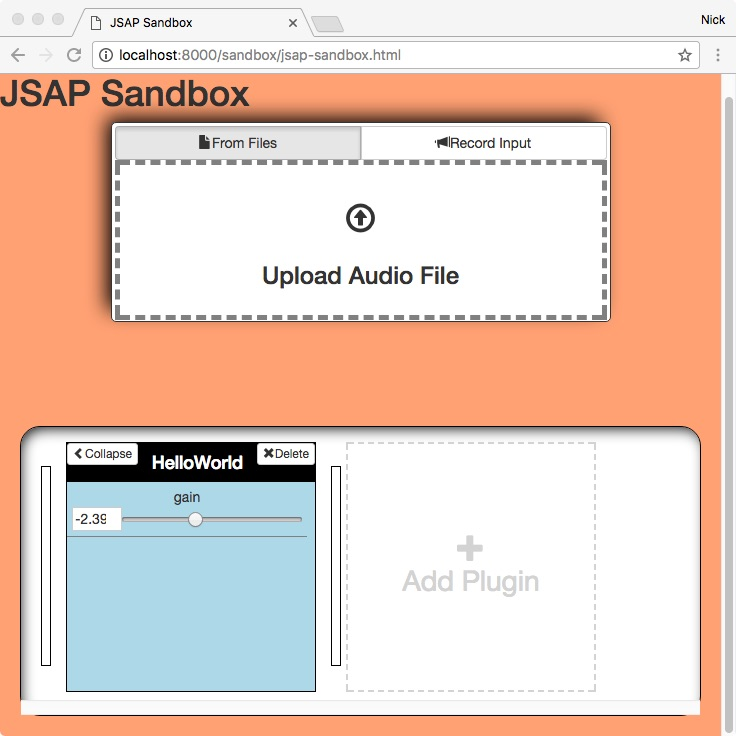
\includegraphics[width=\columnwidth]{final.jpg}
\end{column}
\end{columns}
\end{frame}

\begin{frame}[fragile]
\frametitle{Loading the plugin}
\begin{columns}
\begin{column}{0.4\textwidth}
\begin{enumerate}
\item Get the plugin prototypes
\item Select the prototype you want from that list by the name
\item Call on the chain to load this script into the end of the chain
\end{enumerate}
\end{column}
\begin{column}{0.6\textwidth}
\begin{lstlisting}[language=javascript]
var prototypes = Factory.getProtoypes()
var protoype = prototypes.find(function(a){return a.name == "HelloWorld";});
chain.createPlugin(prototype);
\end{lstlisting}

\end{column}
\end{columns}

\end{frame}

\begin{frame}
\frametitle{Mission accomplished!}
You've now succesfully built and deployed a JSAP instance! Go and make more!\\
You can push any plugins that you make to a reposity of open-source effects at \url{https://github.com/nickjillings/jsap-plugins}.\\
\end{frame}

\begin{frame}
\frametitle{Mission accomplished!}
Further resources:
\begin{itemize}
\item Repositories
\begin{itemize}
\item JSAP: \url{https://github.com/nickjillings/jsap} - Latest versions, issue/buglist
\item JSAP-Plugins: \url{https://github.com/nickjillings/jsap-plugins} - Latest versions, issue/buglist
\end{itemize}
\item Documentation: \url{http://dmtlab.bcu.ac.uk/nickjillings/docs/index.php?src=jsap/index.md}
\item News: \url{http://www.semanticaudio.co.uk/projects/jsap/}
\end{itemize}
\end{frame}

\end{document}